% This must be in the first 5 lines to tell arXiv to use pdfLaTeX, which is strongly recommended.
% In particular, the hyperref package requires pdfLaTeX in order to break URLs across lines.

\documentclass[11pt]{article}
\pagestyle{plain}
\usepackage{fontspec}
\usepackage{tipa} % IPA package
\setmainfont{Times New Roman}
\newfontfamily\ipafont{Charis SIL}
\newcommand{\ipa}[1]{{\ipafont #1}}

\usepackage{array}
\usepackage{booktabs}
\usepackage{caption}
\usepackage{graphicx}
\usepackage{amsmath}
% Remove the "review" option to generate the final version.
\usepackage[final]{ACL2023}

% Standard package includes
\usepackage{times}
\usepackage{latexsym}

% For proper rendering and hyphenation of words containing Latin characters (including in bib files)
\usepackage[T1]{fontenc}
% For Vietnamese characters
% \usepackage[T5]{fontenc}
% See https://www.latex-project.org/help/documentation/encguide.pdf for other character sets

% This assumes your files are encoded as UTF8
\usepackage[utf8]{inputenc}

% This is not strictly necessary, and may be commented out.
% However, it will improve the layout of the manuscript,
% and will typically save some space.
\usepackage{microtype}

% This is also not strictly necessary, and may be commented out.
% However, it will improve the aesthetics of text in
% the typewriter font.
\usepackage{inconsolata}


% If the title and author information does not fit in the area allocated, uncomment the following
%
%\setlength\titlebox{<dim>}
%
% and set <dim> to something 5cm or larger.

\title{Zero-Shot Cross-lingual Phoneme Recognition from Yoruba to English}

\author{Aaron Bahr, Nikita L. Beklemishev, Haejin Cho, Kai Seidenspinner \and Ilinca Vandici \\
         Universtität Tübingen }

\begin{document}
\pdfoutput=1
\maketitle
\outauthor
\begin{abstract}
In this paper, we pre-train an acoustic phoneme recognition model on the TIMIT dataset and evaluate its performance on the Yoruba portion of the Common voice data. We make use of the CTC architecture, allowing us to forego the need for time-aligned input data, and examine the model’s performance after transfer through a thorough and linguistically motivated feature weighting metric. Finally, we look at the phone embeddings produced by our model and try to disentangle training errors from transfer errors. All codes are available in our \href{https://github.com/lilovyjgrib/X-lingual_IPA_ASR}{Github}.
\end{abstract}

\section{Introduction}
Efficiently training an ASR system requires a rich, ideally time-aligned dataset. For low-resource languages, despite efforts towards documentation, exploiting the properties of transfer learning by pre-training on another, high-resource, language remains a sensible option. In our case, we focus solely on producing a consistent, generalized phonemic transcription, conditioned only on acoustic segment (no language model is included). For the purpose of zero-shot evaluation, picking a set of languages with similar phoneme inventories remains the practice yielding the best performance. We chose to work on transferring American English (< West Germanic < Indo-European) to Yoruba (< Volta-Niger < Atlantic-Congo), primarily spoken in Nigeria, whose phoneme inventories overlap to a large extent, despite different areas and \textit{phyla}.
Along with obtaining good performance on both languages, we aim to propose an efficient evaluation metric by employing a linguistically sound feature-weighted version of PER.
Additionally, we also had to tackle the challenge of using non-time-aligned data. While the dataset we used for pre-training offered time-aligned transcriptions, this was not the case for the Yoruba dataset. We opted for an architecture integrating the \textit{Connectionist Temporal Classification Loss}, discarding the time-aligned annotations to make sure we could evaluate on non-time-aligned datasets in the future.

\subsection{English Yoruba Transfer}
\paragraph{Theoretical Capabilities} Successful transfer of knowledge in ASR relies on the fact that languages sound similar. However, acoustic sound is just the input part of the model. A common \textbf{function} from the sound to the tagret sequence is the necessary condition. If the target sequences are words, the model will not be able to transfer, assuming the arbitrariness of the sign. Orthographic symbols are closer, but are not necessarily common between languages. Luckily, for linguistics, the relevant representation of speech is phonemes, which tend to correspond to sound types -- which are, by and large, common. Out of all the sounds that the vocal tract can produce, languages use only a small subset, and some sounds are much more common than others. [Hayes 2009: 6] The shared knowledge of sound types can be described using IPA symbols. [Ladefoged 2011] The model in the present study utilizes this knowledge, by training to write down sentences in IPA [link], [example], further referred to as phonemes, only for simplicity.[link] For example, it should be possible to correctly transcribe this sequence. [edgy example]  Furthermore, by analyzing \textbf{confusion and correspondence} patterns of the function from acoustics to phonemes inherited from English, when applied to Yoruba, we shed light on the variation and universals in these phonological systems. We evaluate the overall performance in section [ref], and this mapping in section [ref].

\paragraph{Expected mismatches} The phonemic systems of Yoruba and English are not exactly similar. This is evident just by IPA inventories, described in Appendix, cf. \cite{Adesola2024}\cite{AhiaEtAl2024}\cite{moran2014} However, a few things are worthy of pointing out. (1) IPA describes the target -- and doesn't show where exactly the border between allophones of one sound and different sounds lies. As such, we can expect that nasal i in Yoruba will be acoustically closer to English e, than i, getting misclassified. To conclude, «placing IPA symbols between slant lines does not in itself designate a unique phonemic analysis» \cite*{vanderhulst2017} E and Y are expected to show a lot of mismatches in the partition of vowel space. (2) Double-articulated /kp/, /gb/ and nasal vowels can also be mapped to sequences of sounds: e.g. /kp/ or /in/. (3) While sound inventories share a lot of similarity, their distribution arises from phonological/phonotactic constraints, which are not as universal \cite{maddieson2010}. An ASR model, meanwhile, includes an RNN, which relies on learning the transition probabilities between classes. For example, English frequent diphthongs make the vowel--glide sequences much more probable than they should be. Yoruba has a constraint for open syllables, which are less likely in English. It would also be interesting to see how the vowel harmony present in Yoruba noises the predictions. (4) Ideally, the model should learn the contrasts of Yoruba. Instead it is trained to learn English distinctions. [] For example, n and l are allophonic in Yoruba. Since they are different phonemes in English, the unnecessary distinction appears. Another example are the approximant and tap r, which are allophones in Yoruba, but belong to /r/ and /t/ in English. The shallow English transcription distinguishes allophones like \ipa{/ɨ/} and \ipa{/i/}, and such cases will further the 1-to-1 correspondence between the model predictions and Yoruba.

\paragraph{Empirical Realisation} Given the differences in inventories discussed above, relating English IPA predictions to Yoruba IPA gold standard becomes a problem: how to say that sequences match, if the alphabet is only in part common? In quantitative spirit of this course,
we define the `sameness' of two phonemes as a gradient from 0 to 1. To find it we can utilize the phonological feature theory [quote].
Each sound has a feature representation, showing which natural classes it belongs and doesn't belong to. Although sounds vary in how much features from the overall set they specify, it is convenient to represent each sound as a vector over the whole feature set,
showing if the feature is positive (+1), negative (-1) or unspecified (0). Then, the Hamming distance of the vectors of with non-0 dimensions, normalised by the length of the dimensionality is the dissimilarity measure. This approach have been widely used before by []. Among many notable databanks aggregating the knowledge of features, such as PHOIBLE \cite{moran2014} and SoundVector[], we chose PanPhon \cite{mortensen2016} for the balance between the quality of representation and availability. The details of the implementation are discussed in Section [ref].

\section{Dataset}
\paragraph{Training set} For training we use the infamous TIMIT ASR corups. \cite{garofolo1993timit} includes 6300 utterances recorded by 630 speakers from 8 major English dialects across the US. Annotations were done according to the customized IPA convention based on ARPAbet \cite{cmudict} (please refer to Appendix \ref{sec:appendix}). As both English and Yoruba are pluricentric languages, the learning benefits a lot from the variety in the input data. Even though TIMIT confines itself to the 1980s US language roof, it represents the existing dialectal variation well. This phonetic variation is necessary for learning to generalize over acoustically different speech sound, which is particularly relevant for transfer learning. Another reason for TIMIT is the popularity of it in ASR studies, which gives us confidence in yielding baseline results, comparable with other works in the area.

\paragraph{Preprocessing the training set} For usage, we first concatenated the train, validation, and test sets and then again randomly split it into train and validation sets with the proportion being 0.25. Thus TIMIT is used only for training and validation in our cross-lingual task. Regarding the audio data, we have extracted log-mel features (dimension 39). The TIMIT alphabet contained 63 unique labels in total. To reduce prediction complexity and to make the phonemic representation of English compatible with that of Yoruba, before mapping to IPA, we merged or split several labels. This included allophones not annotated in the Yoruba corpus: \ipa{<ax-h> /ə̥/} and \ipa{/ə/}, syllabic sonorants, e.g. \ipa{<eng> /ŋ̍/} and \ipa{/ŋ/}. Closures \ipa{<dcl> /d̚ /} and the following releases \ipa{/d/} were joined into one label. In the end, 15 label types were merged. We did not expect systematic unreleased closures in \textbf{open-syllable} Yoruba. \cite{Adesola2024} As for the splitting the combinatorially large inventory of English diphthongs, we split them into vowel--glide sequences, keeping the vowels from the IPA convention: thus \ipa{<oy> /ɔɪ/} became \ipa{<ao y> /ɔ j/}. This step was necessary since Yoruba does not have diphthong vowels. \citet{Przezdziecki2005} We also concluded that splitting vowels will not perplex the prediction given that the CTC decoding does not need time alignment, and our evaluation ignores word boundaries.

\paragraph{Evaluation set} Common Voice Yoruba data was used as a test dataset. Common Voice is a multilingual crowd-sourced corpus aimed for Speech Recognition purposes. \cite{Ardila2020} The audios were recorded by certified native speakers of each language. Annotations are suggested and later validated by other native speaker users via votes.There are 3.4k samples in total and each sample includes an MP3 file, speaker ID and audio transcription written in Yoruba orthography. The dataset also includes data from different dialects. This allows to acknowledge the performance gaps that are shown to arise between standard Yoruba and other dialects in NLP tasks. \citet{AhiaEtAl2024}
\paragraph{Processing the evaluation set} The sets of train (1.4k), validation (913) and test (1.1k) were again concatenated and used together for testing. We kept the original threshold of down votes for invalidated samples. Since we need to keep the shape and content of the train and test data identical, 39-dimensional log-mel feature was extracted from Yoruba in the same way.
We implemented additional grapheme-to-phoneme conversion, since the model predicts IPA symbols given audio inputs, which means that data should at least have phoneme/phonetic representations as a label. We converted Yoruba sentences line-by-line via \texttt{Epitran} Python module. First of all, the word boundaries, as well as the pauses were removed. We also ignored the tone annotation ({\ipa{˧}, \ipa{˦}, \ipa{˨}), although seeing the transfer abilities could be an interesting branch of research. We have removed the marginally phonemic \ipa{/ɔ̃}, \ipa{ŋ/} from the inventory, merging with their allophones \ipa{/ã/} and \ipa{/n/}. \cite{Przezdziecki2005} Another marginal \ipa{/ɛ̃/} remained. The data also turned out to contain an occurrence of dialectal \ipa{<ụ> /ʊ/} \citet{AllenPulleyblankAjiboye2013}, which is too small to generalize from, so we removed it as well from the evaluation for clarity. Full and adjusted Yoruba IPA inventory in Appendix \ref{sec:appendixb}.

\section{Model and Traning}
\subsection{ResNet-Bi-LSTM model}
Our model is based on that of \cite{dhakal2022automatic}, which used ResNet-BiLSTM model for Nepali Speech Recognition. The reason why we chose this model as our base reference was (1) to use pure neural-network-based model so that it is rather easy to train and light-weight in terms of memory, (2) to include residual connection which is largely used in transformers as well as deep neural network models, and (3) to explore whether a model that is trained from scratch can also perform well on zero-shot cross-lingual speech recognition task.

The model starts with 1D-convolution block followed by 1D-Batch Normalization. 5 residual blocks again follows it. This initial CNN layer and ResNet aim to capture locally dependent features and we will call these sets of layers a \emph{ResNet Encoder}. All convolutions are done using identical parameter setting. The kernel size is 15 and the number of channels are 50. Stride is one and dropout rate is 0.2. For residual network encoder, it has 5 residual blocks. Each block consists of 2 unit blocks and one unit block is comprised of initial convolution, Batch Normalization, and PReLU as an activation. Key part of residual block is to add original input to activation layer output. \cite{ravanelli2019speakerrecognitionrawwaveform} have attested that residual connections noticeably stabilize and optimize deep neural network training. It works consistently well with audio task although it was first introduced for image recognition task as can be seen in \cite{dhakal2022automatic}. Another important part of the base model is that it does not include pooling layer. Pooling layers aim to reduce spatial dimension in 2D Convolution setting, so width and height of a feature map would be reduced. In our case, pooling in 1D Convolution would down-sample feature map across time-step and it seems like authors of \cite{dhakal2022automatic} concluded that it is unnecessary to down-sample data across time-step. Bi-LSTM encoder part then follows residual networks. Bi-LSTM is designed to reflect distinctive contextual features in two opposite directions. \cite{dhakal2022automatic} has two RNN layers with its dimension being both 170. As final layers, two dense layers and ReLU activation takes the output of bi-LSTM and maps 170-dimension input into 66-dimension output data. 66-dimension is set based on the number of labels in Nepali inventory.

We have mostly followed \cite{dhakal2022automatic}'s model design. However we did make several key changes to prevent overfitting and to keep the depth of our model shallower so that our model can be applicable for cross-lingual inference. Each adjustments is based on our experiments, but unfortunately we did not properly record the difference for each inspections. (1) The first major change is to reduce the depth of ResNet encoder block. Our model has 3 residual blocks while the original model has 5 blocks. Also, one residual block has only one set of unit block while the original residual block has 2 unit blocks. In other words, our ResNet encoder part is 0.3 times depth of that of the base model ResNet encoder. All other settings regarding ResNet encoder have fixed same as \cite{dhakal2022automatic}. (2) We have also diminished hidden dimensions of Bi-LSTM encoder and dense layer. From 170 to 128 as to hidden dimension of RNN layer and from 340 to 256 as to dense layer dimension. This also contributes to better computational efficiency as it corresponds to GPU's natural memory alignment and fetches. (3) Last but not least, we have introduced saliently strong dropout rate for RNN layers. 0.4 was adopted as dropout rate. This was also part of an effort to enable cross-lingual application. Refer to following visualization marks key difference between \cite{dhakal2022automatic} and our model.
Learning without an LM CTC.
\begin{figure}
    \centering
    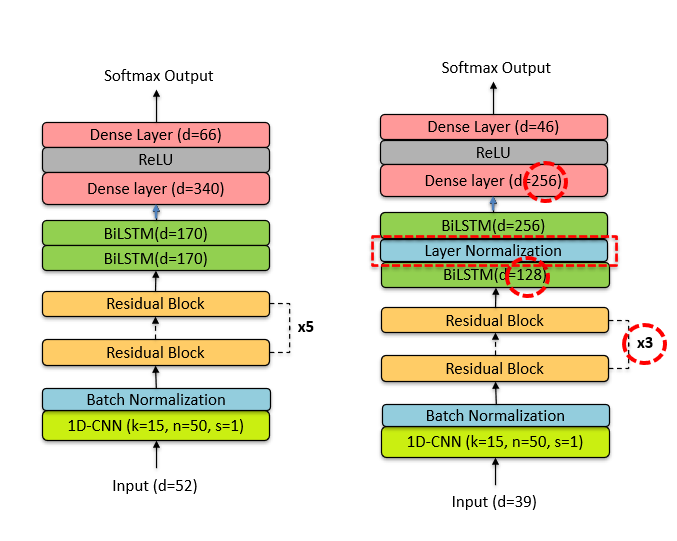
\includegraphics[width=1\linewidth]{modelarchitecture+.png}
    \caption{Left: model architecture of \cite{dhakal2022automatic} , Right: Adjusted model architecture for English-Yoruba cross-lingual phoneme recognition. Changes highlighted with a red circle.}
    \label{fig:architecture}
\end{figure}


\begin{figure}
    \centering
    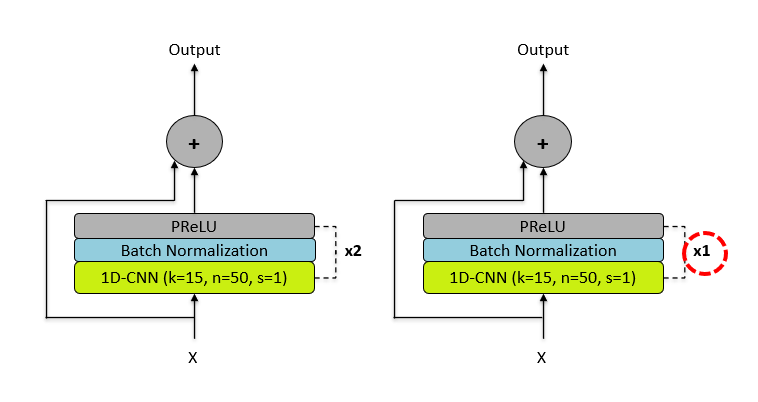
\includegraphics[width=1\linewidth]{residualblock.PNG}
    \caption{Left: residual block of \cite{dhakal2022automatic}, Right: Adjusted residual block for English-Yoruba cross-lingual phoneme recognition. Changes highlighted with a red circle.}
    \label{fig:residualblock}
\end{figure}

We employed Connectionist Temporal Classification (CTC) loss as our training criterion. Unlike conventional frame-level cross-entropy, CTC does not require pre-aligned input-label pairs, which makes it especially suitable for low-resource languages such as Yoruba, where alignment information is unavailable. The key idea of CTC is to introduce a blank symbol and permit label repetitions so that multiple frame-level alignments can correspond to the same output sequence. During training, CTC computes the negative log-likelihood of the target sequence by summing the probabilities of all valid alignments:
$$L_{CTC} = \sum_{(X, Y) \in D} - \log P_{CTC}(Y \mid X)$$
where the probability of a target sequence $Y$ given the input $X$ is defined as
\[
\begin{aligned}
P_{CTC}(Y \mid X) &= \sum_{A \in B^{-1}(Y)} P(A \mid X) \\
                  &= \sum_{A \in B^{-1}(Y)} \prod_{t=1}^{T} p(a_t \mid h_t)
\end{aligned}
\]
with $A=(a_1, \dots, a_T)$ being a frame-level alignment, $B$ the collapse function that removes blanks and repeated labels, and $h_t$ the hidden representation at time $t$. The blank symbol $\epsilon$ needs to be manually added to the alphabet so that the model can output blanks during training and inference.

At decoding time, greedy decoding selects the most probable label at each timestep, and the CTC collapse operation removes duplicates and blanks to produce the final prediction sequence $\hat{Y}$.
$$\hat{Y} = \arg\max_{Y} P_{CTC}(Y \mid X).$$

\subsection{Train}
Train settings were set through multiple experiments. The number of epochs is 50 and batch size was 64. We have adopted Adam as our stochastic gradient optimizer and set weight decay as 1e-4. A plateau-based learning rate scheduler was used and the initial learning rate was 1e-3. The total number of parameters are 0.8 million. With (hyper)parameter settings given above, training was noticeably stable and robust to overfitting. Both training and validation loss and PER consistently decreased and we halted training at the 16th epoch where Train PER reached 0.0223 and Validation PER reached a similar figure, 0.0339.

\section{Results}

\textbf{text result - PER, ACC}
\begin{figure}
    \centering
    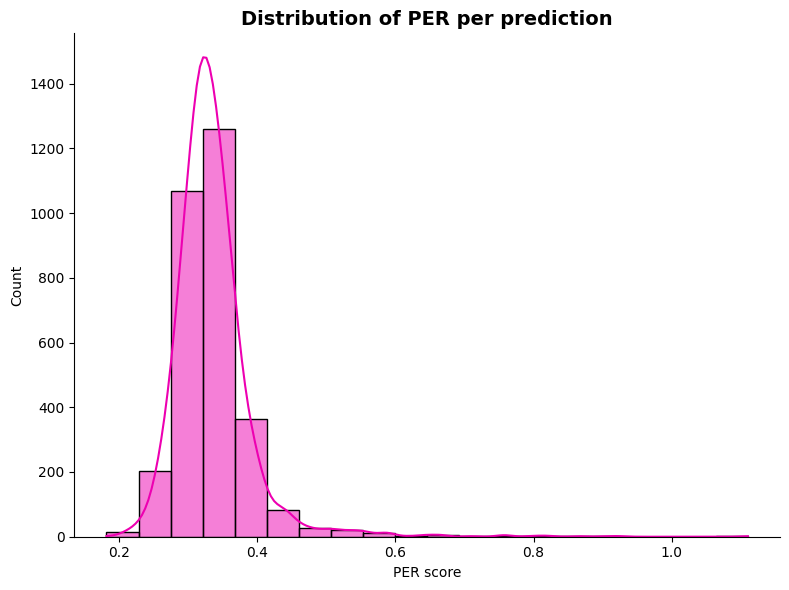
\includegraphics[width=0.75\linewidth]{model_per_distribution.png}
    \caption{PER Distribution}
    \label{fig:placeholder}
\end{figure}

To evaluate the output of our model on Yoruba, we have to adjust the Phoneme Error Rate for the issue of different IPA inventories. [ref intro] The metric we employ is feature-weighted PER. Like the regular PER, Levenshtein algorithm, with deletion, insertion and substitution operations. Special attention is given to the substitution operation, where the cost is determined by a feature-weighting scheme (which we derive from the PanPhon package). To obtain these measures, we convert the ARPA characters to IPA, thereby not directly evaluating on raw output. During inference, we observed that our model had a tendency to overgenerate, making the output consistently longer than the gold labels. Lowering the deletion cost from 0.75 to 0.5 helped improve this. However, we still keep this issue in mind for later discussion.

Default PER was 0.34 without any adjustment on deletion, insertion, and substitution operations. PER distribution graph draws positively-skewed bell curve. Together with equi-weighted features and deletion still set as 1.0, PER decreased to 0.35. As mentioned above, adapting deletion cost from 1.0 to 0.5 made the metric even lower to 0.33.

\begin{figure}
    \centering
    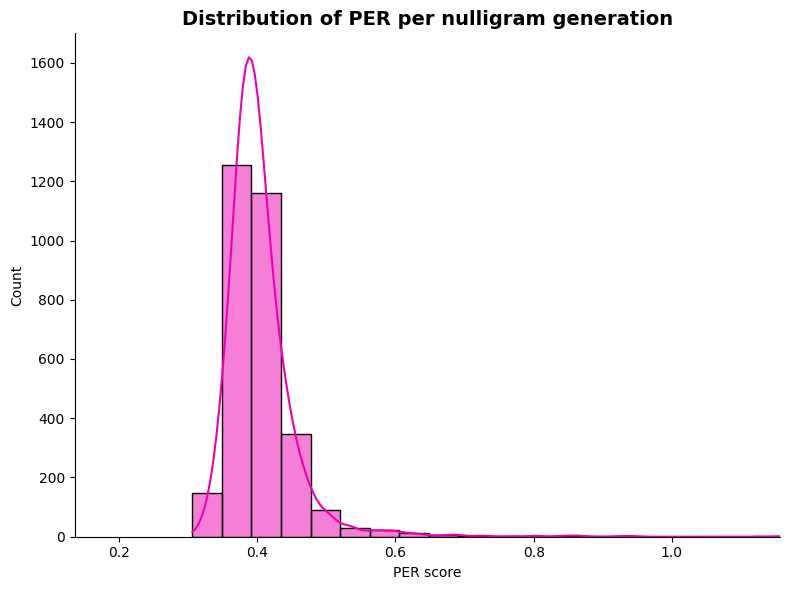
\includegraphics[width=0.75\linewidth]{nulligram_PER_distribution.png}
    \caption{Equal probability PER Distribution}
    \label{fig:placeholder}
\end{figure}
Nulligram PER is further investigated by artifically creating a Yoruba nulligram in which the order of phonemes was randomized. The aim was to examine whether co-occurrence patterns of certain phonemes influence model performance. If the PER of nulli-gram corpus is higher than that of default PER, it suggests that phoneme collocation contributes positively to phoneme recognition. At the very least, it would indicate that the naturally occurring co-occurrence patterns are not so complex as to hinder recognition performance.

Nulligram PER was reported to be 0.36, which is 0.2 higher than default PER. This would in turn suggest that natural sequential distribution of phonemes helps predicting them.
\begin{figure}
    \centering
    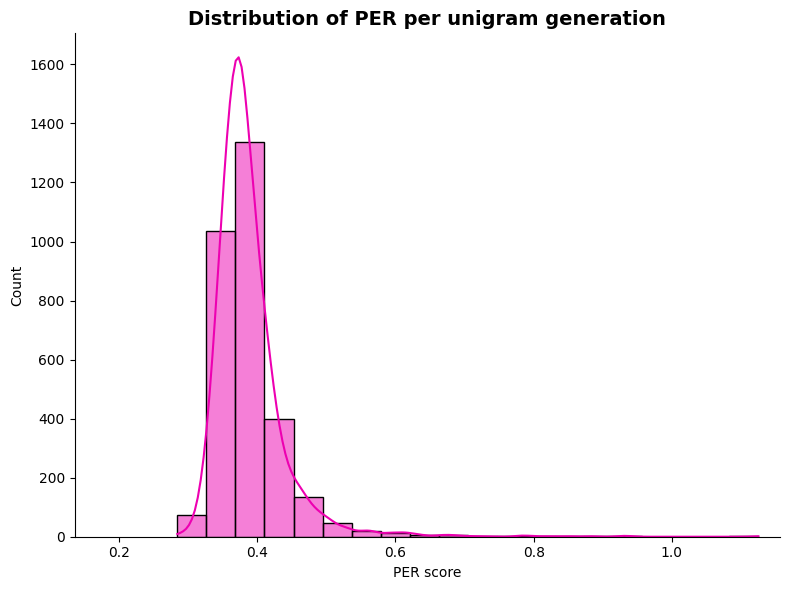
\includegraphics[width=0.75\linewidth]{unigram_PER_distribution.png}
    \caption{Unigram PER Distribution}
    \label{fig:placeholder}
\end{figure}

\subsection{Inference}

\subsection{Phone Embeddings Extraction}
We later experiment with inference to produce phone embeddings, and attempt to plot these using dimensionality reduction. We collect the final embeddings for each correctly predicted phoneme (whose feature size length equals the vocabulary size) and use UMAP to obtain 2 dimensional embeddings, for which we obtain the mean by phoneme. We settled on UMAP since it maintain the non-linear assumption of t-SNE regarding the data while being less dependent on initialization. Note that we converted the labels obtained by inference to IPA for ease of comparison. While both plots seem to group similar sounds together to an extent (e.g), comparing inference simultaneously on both datasets remains tricky due to 1) the different probability distributions, and, to an extent, the different in dataset sizes 2) while UMAP remains an efficient dimensionality reduction method, it is unclear whether plotting always reflects similarity through clustering.
To investigate this further, we decided to run a correlation test between the Euclidian distance between phones (after dimensionality reduction) and feature weight. This shows that there is a significant correlation between the two variables, but it presents a low, negative regression coefficients, showing that phonemes with different features tend to have a relative larger Euclidian value, which goes against what we would initially hope for. Moreover, attempting to map mean Yoruba and English embeddings into the same space and then computing their distance across several trials shows a high degree of variation.

We can see that in some cases, similar sounds do tend to cluster, but these patterns seem to differ from language to language. For Yoruba, we can observe vowels clustering together
in the same part of the space, while consonants remain together. The sibilants /textipa{s} and /textipa{S} seemed to be the closest pair in that space, possibly indicating that the model's embedding space reflects similarity between these.
But in the case of the other consonants, it is more difficult to establish a clear-cut pattern, although we could argue that there is a delineation between voiced and unvoiced consontants.
As for the projection obtained by TIMIT, it also seems that only a few patterns are reflected in the space, for instance /textipa{i} and  /textipa{I}, although all of the vowels are not grouped within the same space.

We also look into the simultaneous projection of Yoruba and English embeddings in the same space, by first fitting the transform based on the English data, and then reducing the Yoruba data, collecting
Euclidian distances between the common phonemes. After running the projection several times, we find that the distances we obtain are consistent accross trials, but it is difficult to extract a common pattern.

Since projections obtained through UMAP tend to be hard to interpret, we then look into whether the Euclidian distance between phonemes in the reduced dimensional space can correlated to the feature weighing scheme we implemented.
We find that these variables have a significant p-value for both datasets, and are positively correlated. Since no definite overarching pattern can be established the actual embeddings, we posit that this might be due to the distribution of phonemes in the data,
and leave the elaboration to further studies. 	

\subsection{Discussions}

We obtain posterior probabilities of prediction labels based on gold labels (see Figure 7). At a first glance, we can see predictions close to the gold label tend to have a higher probability. For the majority labels for which the most common prediction is incorrect, it usually still reflects a degree of similarity with the most common label (for instance, i is the most likely prediction for e).

\begin{figure}
    \centering
    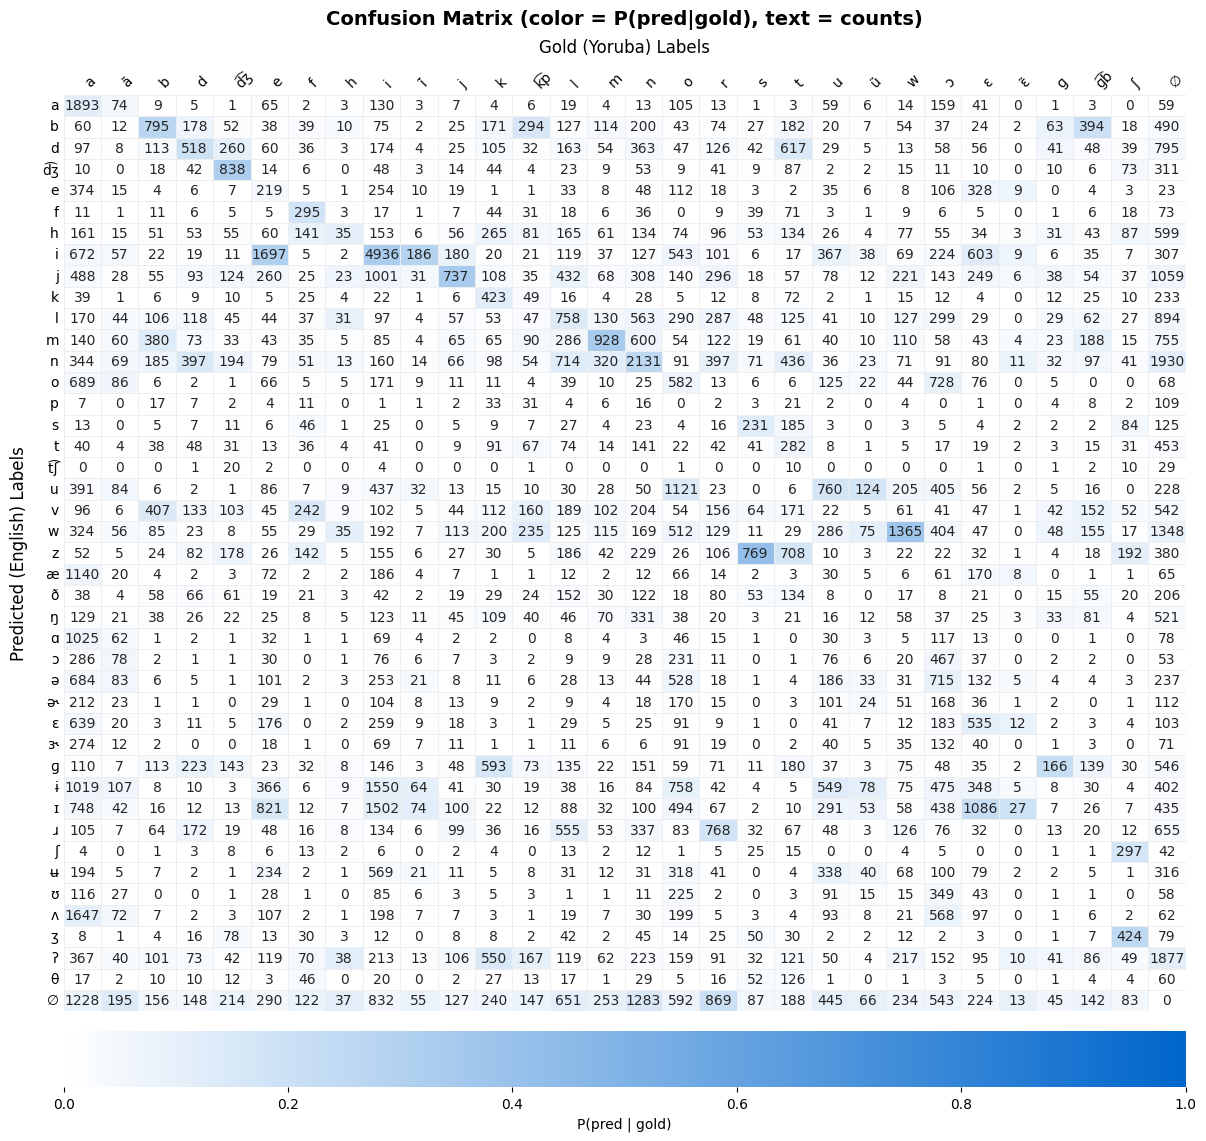
\includegraphics[width=1\linewidth]{EngYorConfusionMatrix.png}
    \caption{English-Yoruba Confusion Matrix with Posterior Probability}
    \label{fig:placeholder}
\end{figure}

- yoruba phoneme frequency
\begin{figure}
    \centering
 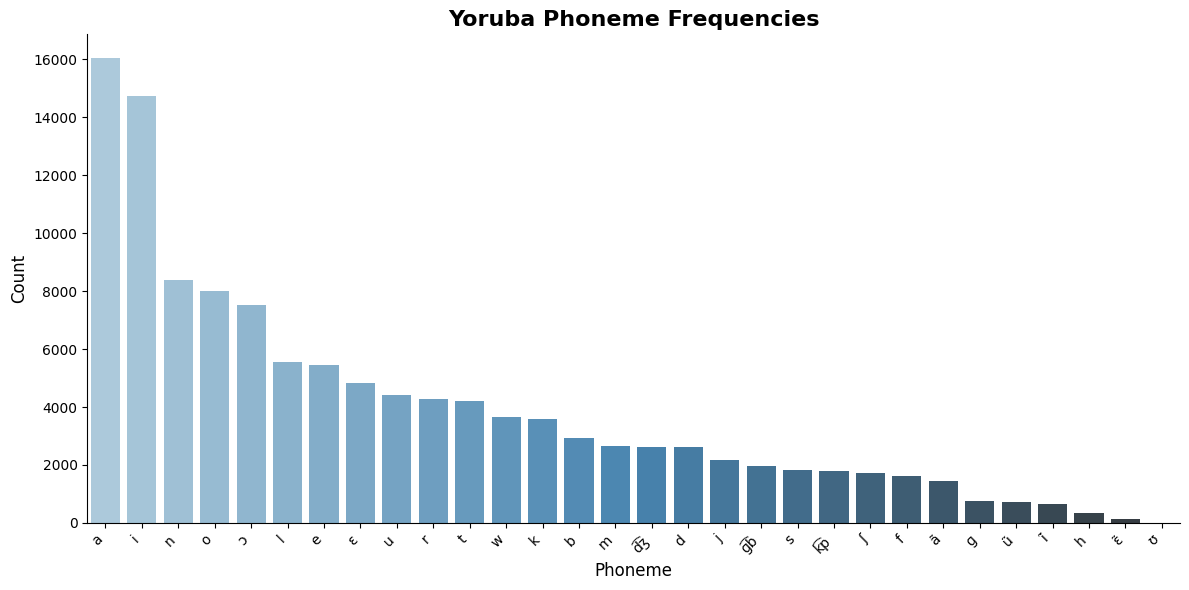
\includegraphics[width=1\linewidth]{YorPhonemeFrequency.png}
    \caption{Yoruba Phoneme Frequency}
    \label{fig:placeholder}
\end{figure}



- Normalized PMI
\begin{figure}
    \centering
    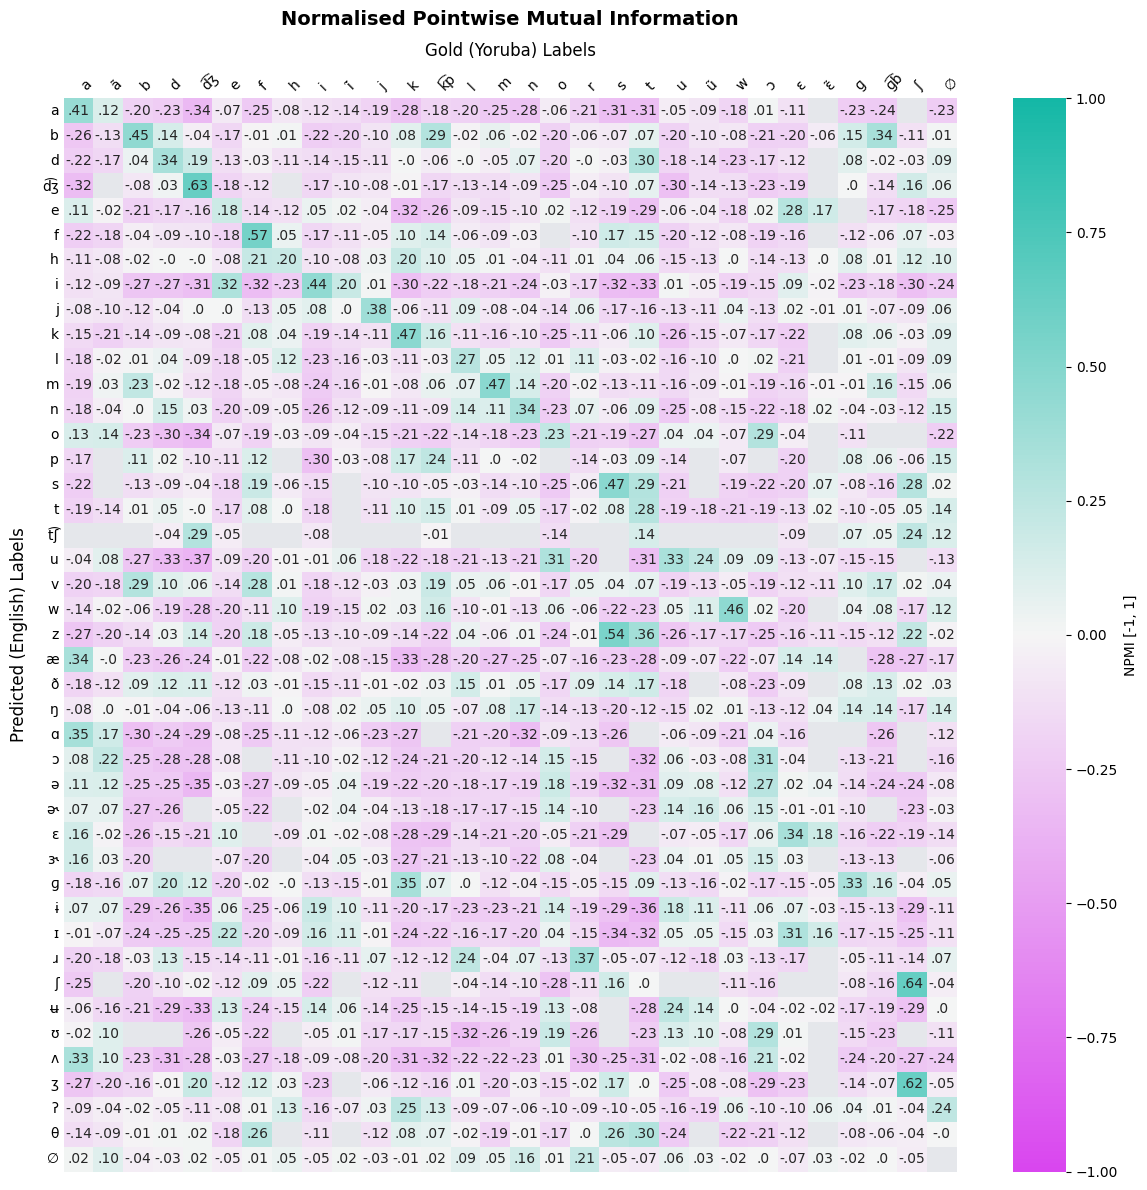
\includegraphics[width=1\linewidth]{NormalisedPMI.png}
    \caption{Normalized PMI}
    \label{fig:placeholder}
\end{figure}

- confusion entropy
\begin{table}[h!]
\centering
\caption{Confusion Entropy}
\begin{tabular}{lc}
\toprule
\textbf{Label} & \textbf{H} \\
\midrule
\ipa{∅}    & 4.64 \\
\ipa{ã}   & 4.55 \\
\ipa{ɔ}    & 4.53 \\
\ipa{a}    & 4.52 \\
\ipa{o}    & 4.41 \\
\ipa{h}    & 4.33 \\
\ipa{l}    & 4.26 \\
\ipa{ũ}   & 4.21 \\
\ipa{k͡p}  & 4.18 \\
\ipa{ɡ}    & 4.18 \\
\ipa{t}    & 4.16 \\
\ipa{u}    & 4.16 \\
\ipa{f}    & 4.14 \\
\ipa{ɡ͡b}  & 4.13 \\
\ipa{k}    & 4.10 \\
\ipa{ɛ}    & 4.09 \\
\ipa{r}    & 4.07 \\
\ipa{n}    & 4.03 \\
\ipa{d}    & 4.00 \\
\ipa{ɛ̃}   & 3.99 \\
\ipa{ĩ}   & 3.93 \\
\ipa{j}    & 3.92 \\
\ipa{e}    & 3.87 \\
\ipa{w}    & 3.82 \\
\ipa{i}    & 3.81 \\
\ipa{ʃ}    & 3.80 \\
\ipa{b}    & 3.76 \\
\ipa{d͡ʒ}  & 3.69 \\
\ipa{m}    & 3.67 \\
\ipa{s}    & 3.40 \\
\bottomrule
\end{tabular}
\end{table}

\begin{figure}
    \centering
    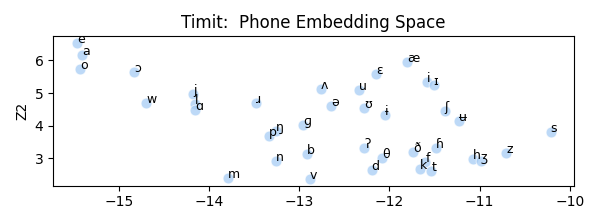
\includegraphics[width=1\linewidth]{timitultphone.png}
    \caption{Timit Phone Embeddings}
    \label{fig:placeholder}
\end{figure}

\begin{figure}
    \centering
    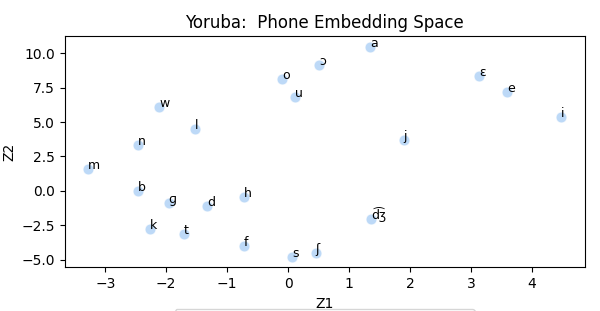
\includegraphics[width=1\linewidth]{yorlast.png}
    \caption{Yoruba Phone Embeddings}
    \label{fig:placeholder}
\end{figure}

\begin{figure}
    \centering
    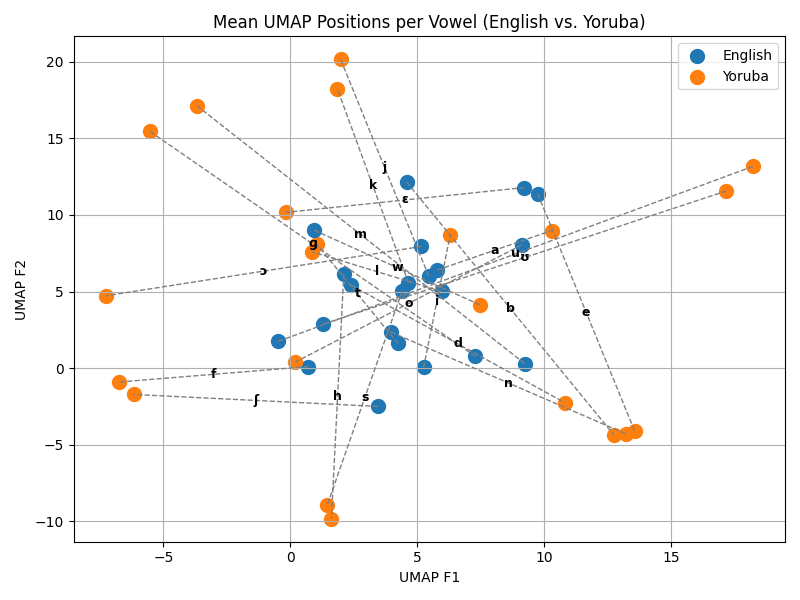
\includegraphics[width=1\linewidth]{yoruba_eng_plot.png}
    \caption{Vowel distances between English and Yoruba}
    \label{fig:placeholder}
\end{figure}

\begin{figure}
    \centering
    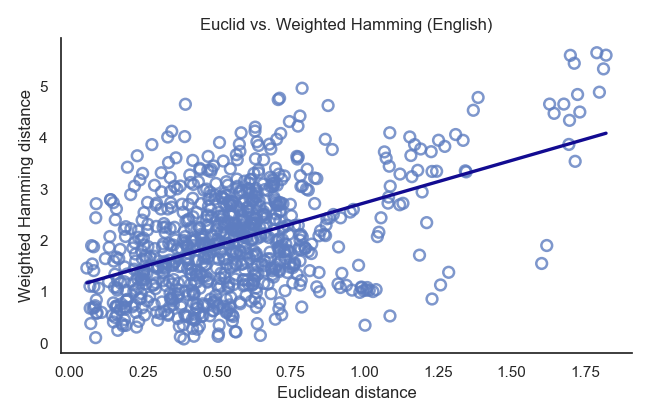
\includegraphics[width=1\linewidth]{timitcor.png}
    \caption{Correlation between Euclidian distance of embeddings and Weighted Hamming distance (English)}
    \label{fig:placeholder}
\end{figure}

\begin{figure}
    \centering
    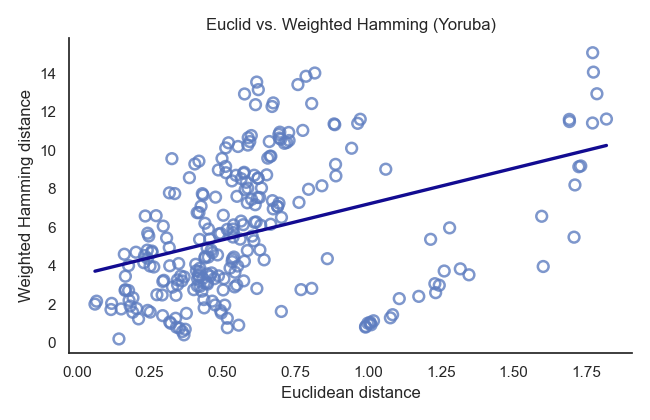
\includegraphics[width=1\linewidth]{yorlastcor.png}
    \caption{Correlation between Euclidian distance of embeddings and Weighted Hamming distance (Yoruba)}
    \label{fig:placeholder}
\end{figure}

\begin{table}[h]
\centering
\caption{Pearson correlation between vowel distance and another variable}
\begin{tabular}{lrr}
\toprule
\textbf{Language} & \textbf{Correlation Coefficient ($r$)} & \textbf{$p$-value} \\
\midrule
English & $0.47$ & $0.0002$ \\
Yoruba  & $0.49$ & $0.004$ \\
\bottomrule
\end{tabular}
\end{table}



\begin{table}
\caption{Vowel distances between English and Yoruba (sorted by similarity)}
\centering
\begin{tabular}{lr}
\toprule
Vowel & Distance \\
\midrule
u & 0.095 \\
ɡ & 0.170 \\
k & 1.119 \\
d & 1.280 \\
m & 1.424 \\
t & 1.571 \\
j & 1.633 \\
s & 1.800 \\
ɔ & 1.947 \\
ɛ & 1.971 \\
b & 1.993 \\
h & 2.549 \\
n & 2.887 \\
w & 2.907 \\
					
e & 3.059 \\
ʃ & 3.278 \\
o & 3.291 \\
l & 3.363 \\
i & 3.590 \\
a & 3.643 \\
f & 5.945 \\
\bottomrule
\end{tabular}
\end{table}

\begin{figure}
    \centering
    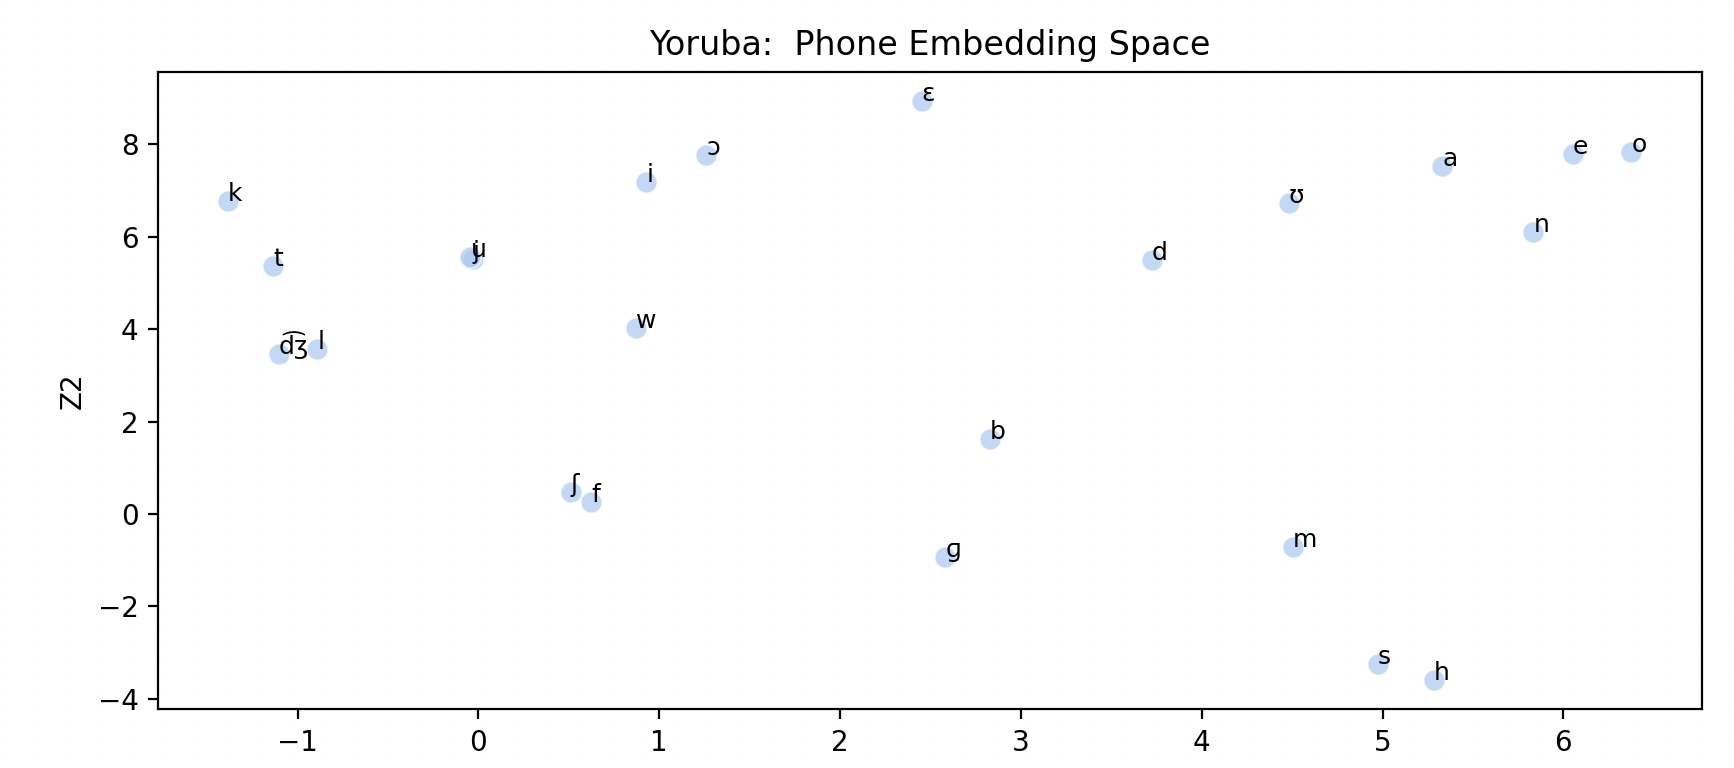
\includegraphics[width=1\linewidth]{Yoruba_Embeddings.png}
    \caption{Yoruba Phone Embeddings}
    \label{fig:placeholder}
\end{figure}

\begin{figure}
    \centering
    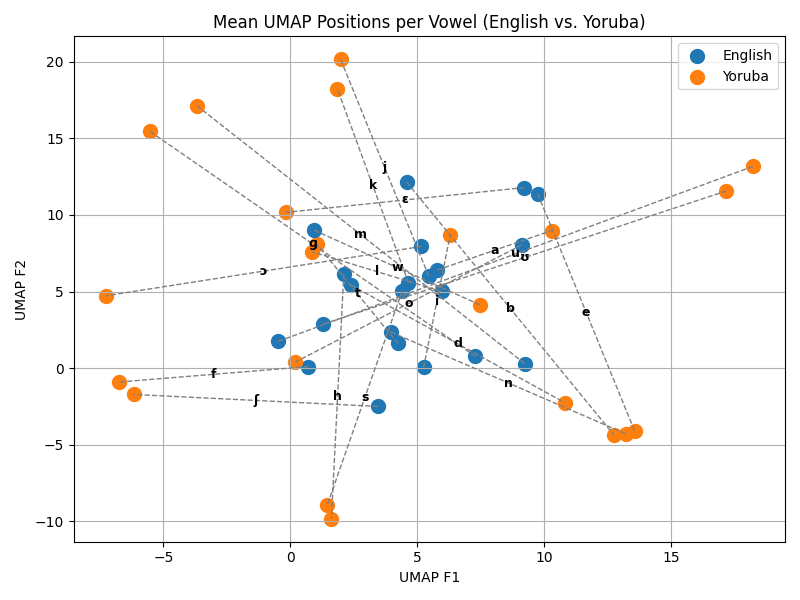
\includegraphics[width=1\linewidth]{yoruba_eng_plot.png}
    \caption{Yoruba and English embeddings plotted in the same space}
    \label{fig:placeholder}
\end{figure}




\section*{Limitations}

For future reference, we believe that our model could be further improved by dedicating more attention to the over-generation problem, and possibly address it at the pre-training stage with a modified pre-training objective, or by investigating whether there are some repeating patterns linked to over-generation. This would then in turn help improve the quality of alignment for the evaluation step.
As we did not keep track of the train-test split, the impact that this has on the evaluation step is unclear. Re-producing it with a proper split might yield more comprehensible results, especially when it comes to posterior probabilities.
We also encourage the reproduction of this study on different datasets, be it for Yoruba or other languages.


\bibliographystyle{plain}
\bibliography{xlingualreference}


\appendix
\section{Appendix}
\label{sec:appendix}
\subsection{Appendix. A}

\begin{table}[h!]
\centering
\caption{TIMIT to IPA mapping}
\begin{tabular}{>{\ttfamily}l >{\ipafont}l> {\ipafont}l}
\toprule
\textbf{TIMIT} & \textbf{IPA} & \textbf{IPA (adjusted)}\\
\midrule
aa   & \ipa{ɑ}   & \ipa{ɑ}\\
ae   & \ipa{æ}   & \ipa{æ}\\
ah   & \ipa{ʌ}   & \ipa{ʌ}\\
ao   & \ipa{ɔ}   & \ipa{ɔ}\\
aw   & \ipa{aw}  & \ipa{a + w}\\
ay   & \ipa{aj}  & \ipa{a + j}\\
ax   & \ipa{ə}   & \ipa{ə}\\
axr  & \ipa{ə˞}  & \ipa{ə}\\
eh   & \ipa{ɛ}   & \ipa{ɛ}\\
er   & \ipa{ɜ˞}  & \ipa{ɜ˞}\\
ey   & \ipa{ej}  & \ipa{e + j}\\
ih   & \ipa{ɪ}   & \ipa{ɪ}\\
ix   & \ipa{ɨ}   & \ipa{ɨ}\\
iy   & \ipa{i}   & \ipa{i}\\
ow   & \ipa{ow}  & \ipa{o + w}\\
oy   & \ipa{ɔj}  & \ipa{ɔ + j}\\
uh   & \ipa{ʊ}   & \ipa{ʊ}\\
uw   & \ipa{u}   & \ipa{u}\\
ux   & \ipa{ʉ}   & \ipa{ʉ}\\
ax-h & \ipa{ə̥}  & \ipa{ə}\\
bcl  & \ipa{b̚}  & \ipa{b}\\
dcl  & \ipa{d̚}  & \ipa{d}\\
eng  & \ipa{ŋ̍}  & \ipa{ŋ}\\
gcl  & \ipa{ɡ̚}  & \ipa{g}\\
hv   & \ipa{ɦ}   & \ipa{h}\\
kcl  & \ipa{k̚}  & \ipa{k}\\
pcl  & \ipa{p̚}  & \ipa{p}\\
tcl  & \ipa{t̚}  & \ipa{t}\\
pau  & \ipa{|}   & \ipa{–}\\
epi  & \ipa{||}  & \ipa{–}\\
h\#  & \ipa{/}   & \ipa{–}\\
b    & \ipa{b}   & \ipa{b}\\
ch   & \ipa{t͡ʃ} & \ipa{t͡ʃ}\\
d    & \ipa{d}   & \ipa{d}\\
dh   & \ipa{ð}   & \ipa{ð}\\
dx   & \ipa{ɾ}   & \ipa{r}\\
el   & \ipa{l̩}  & \ipa{l}\\
em   & \ipa{m̩}  & \ipa{m}\\
en   & \ipa{n̩}  & \ipa{n}\\
f    & \ipa{f}   & \ipa{f}\\
g    & \ipa{g}   & \ipa{g}\\
hh   & \ipa{h}   & \ipa{h}\\
h    & \ipa{h}   & \ipa{h}\\
jh   & \ipa{d͡ʒ} & \ipa{d͡ʒ}\\
k    & \ipa{k}   & \ipa{k}\\
l    & \ipa{l}   & \ipa{l}\\
m    & \ipa{m}   & \ipa{m}\\
n    & \ipa{n}   & \ipa{n}\\
nx   & \ipa{ɾ̃}  & \ipa{n}\\
ng   & \ipa{ŋ}   & \ipa{ŋ}\\
p    & \ipa{p}   & \ipa{p}\\
q    & \ipa{ʔ}   & \ipa{ʔ}\\
r    & \ipa{ɹ}   & \ipa{r}\\
s    & \ipa{s}   & \ipa{s}\\
sh   & \ipa{ʃ}   & \ipa{ʃ}\\
t    & \ipa{t}   & \ipa{t}\\
th   & \ipa{θ}   & \ipa{θ}\\
v    & \ipa{v}   & \ipa{v}\\
w    & \ipa{w}   & \ipa{w}\\
wh   & \ipa{ʍ}   & \ipa{ʍ}\\
y    & \ipa{j}   & \ipa{j}\\
z    & \ipa{z}   & \ipa{z}\\
zh   & \ipa{ʒ}   & \ipa{ʒ}\\
\bottomrule
\end{tabular}
\end{table}

\subsection{Appendix. B}
\label{sec:appendixb}
\begin{table}[h!]
\centering
\caption{Yoruba IPA inventory}
\begin{tabular}{>{\itshape}l >{\ipafont}l >{\ipafont}l}
\toprule
\textbf{Yoruba} & \textbf{IPA} & \textbf{IPA (adjusted)}\\
\midrule
m & \ipa{m} & \ipa{m} \\
i & \ipa{i} & \ipa{i} \\
k & \ipa{k} & \ipa{k} \\
y & \ipa{j} & \ipa{j} \\
u & \ipa{u} & \ipa{u} \\
a & \ipa{a} & \ipa{a} \\
w & \ipa{w} & \ipa{w} \\
n & \ipa{n} & \ipa{n} \\
t & \ipa{t} & \ipa{t} \\
l & \ipa{l} & \ipa{l} \\
s & \ipa{s} & \ipa{s} \\
b & \ipa{b} & \ipa{b} \\
e & \ipa{e} & \ipa{e} \\
o & \ipa{o} & \ipa{o} \\
g & \ipa{ɡ} & \ipa{ɡ} \\
h & \ipa{h} & \ipa{h} \\
d & \ipa{d} & \ipa{d} \\
r & \ipa{ɾ} & \ipa{r} \\
f & \ipa{f} & \ipa{f} \\
\d{e} & \ipa{ɛ} & \ipa{ɛ} \\
\d{s} & \ipa{ʃ} & \ipa{ʃ} \\
\d{o} & \ipa{ɔ} & \ipa{ɔ} \\
j & \ipa{d͡ʒ} & \ipa{d͡ʒ} \\
\textasciiacute & \ipa{˦} & \ipa{–} \\
\textasciigrave & \ipa{˨} & \ipa{–} \\
in & \ipa{ĩ} & \ipa{ĩ} \\
un & \ipa{ũ} & \ipa{ũ} \\
gb & \ipa{ɡ͡b} & \ipa{ɡ͡b} \\
p & \ipa{k͡p} & \ipa{k͡p} \\
\d{o}n & \ipa{ɔ̃} & \ipa{ã} \\
\d{e}n & \ipa{ɛ̃} & \ipa{ɛ̃} \\
an & \ipa{ã} & \ipa{ã} \\
-- & \ipa{˧} & \ipa{–} \\
n & \ipa{ŋ} & \ipa{–} \\
\d{u} & \ipa{ʊ} & \ipa{–} \\
\d{i} & \ipa{ɪ} & \ipa{–} \\
\bottomrule
\end{tabular}
\end{table}

\subsection{Appendix. C}

This is a section in the appendix.

\end{document}
